\documentclass[border=3pt]{standalone}
\usepackage{giambattista}
\setmainfont{TeX Gyre Pagella}
\setsansfont{Latin Modern Sans}
\setmonofont[Scale=0.8,Ligatures=NoCommon]{Cavalcade Mono}
\usepackage{mathmacros}
\usepackage[svgnames]{xcolor} 
\usepackage[utf8]{inputenc} 
\usepackage{fullpage}
\usepackage{tikz}
\usetikzlibrary{arrows,calc,
                shapes,positioning}
\thispagestyle{empty}

\begin{document}
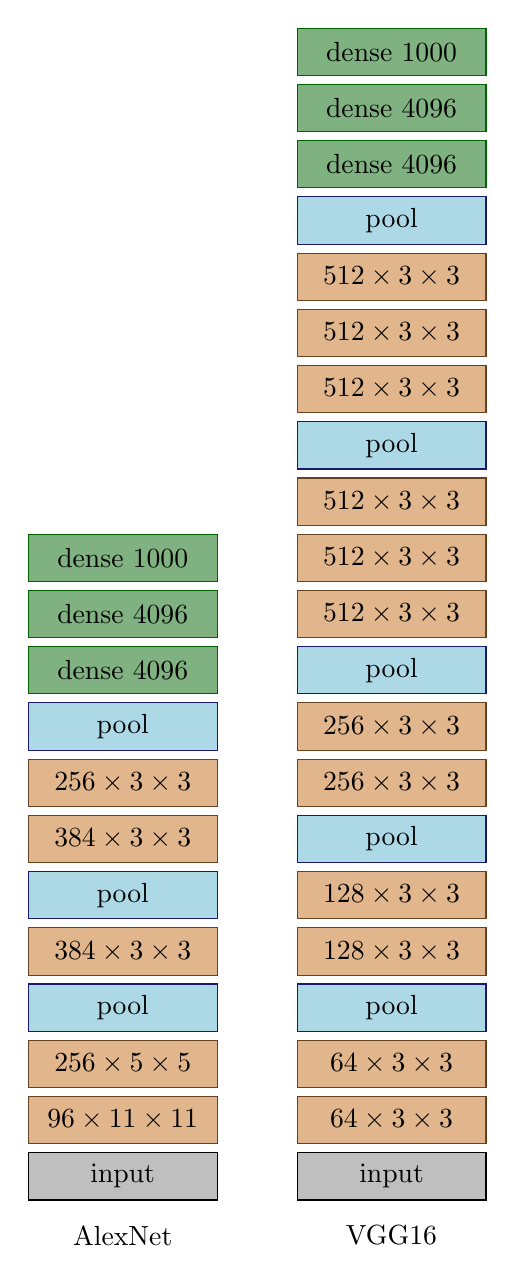
\begin{tikzpicture}
  \tikzset{layer/.style = {shape = rectangle, minimum width = 24mm, minimum height = 6mm}}
  \tikzset{input/.style = {layer, fill = white!50!gray, draw = black}}
  \tikzset{conv/.style = {layer, fill = white!40!Peru, draw = black!50!Peru}}
  \tikzset{pool/.style = {layer, fill = LightBlue, draw = MidnightBlue}}
  \tikzset{dense/.style = {layer, fill = white!50!DarkGreen, draw = DarkGreen}}

  \node[input] (AlexInput) {input};
  \node[below = 2mm of AlexInput] {AlexNet}; 
  \node[conv, above = 1mm of AlexInput] (C1) {$96 \times 11 \times 11$};
  \node[conv, above = 1mm of C1] (C2) {$256 \times 5 \times 5$};
  \node[pool, above = 1mm of C2] (P1) {pool};
  \node[conv, above = 1mm of P1] (C3) {$384 \times 3\times 3$};
  \node[pool, above = 1mm of C3] (P2) {pool};
  \node[conv, above = 1mm of P2] (C4) {$384 \times 3\times 3$};
  \node[conv, above = 1mm of C4] (C5) {$256 \times 3\times 3$};
  \node[pool, above = 1mm of C5] (P3) {pool};
  \node[dense, above = 1mm of P3] (D1) {dense 4096};
  \node[dense, above = 1mm of D1] (D2) {dense 4096};
  \node[dense, above = 1mm of D2] (D3) {dense 1000};

  \node[input, right = of AlexInput] (VGG16Input) {input};
  \node[below = 2mm of VGG16Input] {VGG16}; 
  \node[conv, above = 1mm of VGG16Input] (VC1) {$64 \times 3 \times 3$};
  \node[conv, above = 1mm of VC1] (VC2) {$64 \times 3 \times 3$};
  \node[pool, above = 1mm of VC2] (VP1) {pool};
  \node[conv, above = 1mm of VP1] (VC3) {$128 \times 3\times 3$};
  \node[conv, above = 1mm of VC3] (VC4) {$128 \times 3\times 3$};
  \node[pool, above = 1mm of VC4] (VP2) {pool};
  \node[conv, above = 1mm of VP2] (VC5) {$256 \times 3\times 3$};
  \node[conv, above = 1mm of VC5] (VC6) {$256 \times 3\times 3$};
  \node[pool, above = 1mm of VC6] (VP3) {pool};
  \node[conv, above = 1mm of VP3] (VC7) {$512 \times 3\times 3$};
  \node[conv, above = 1mm of VC7] (VC8) {$512 \times 3\times 3$};
  \node[conv, above = 1mm of VC8] (VC9) {$512 \times 3\times 3$};
  \node[pool, above = 1mm of VC9] (VP4) {pool};
  \node[conv, above = 1mm of VP4] (VC10) {$512 \times 3\times 3$};
  \node[conv, above = 1mm of VC10] (VC11) {$512 \times 3\times 3$};
  \node[conv, above = 1mm of VC11] (VC12) {$512 \times 3\times 3$};
  \node[pool, above = 1mm of VC12] (VP5) {pool};
  \node[dense, above = 1mm of VP5] (VD1) {dense 4096};
  \node[dense, above = 1mm of VD1] (VD2) {dense 4096};
  \node[dense, above = 1mm of VD2] (VD3) {dense 1000};

\end{tikzpicture}
\end{document}
